\documentclass{standalone}
\usepackage{tikz}
\usetikzlibrary{patterns}
\usetikzlibrary{positioning}
\usetikzlibrary{patterns, positioning}
\usetikzlibrary{shapes.misc}
\usepackage[outline]{contour}
\contourlength{1.5pt} 
\usepackage[sfdefault]{ClearSans}

\begin{document}
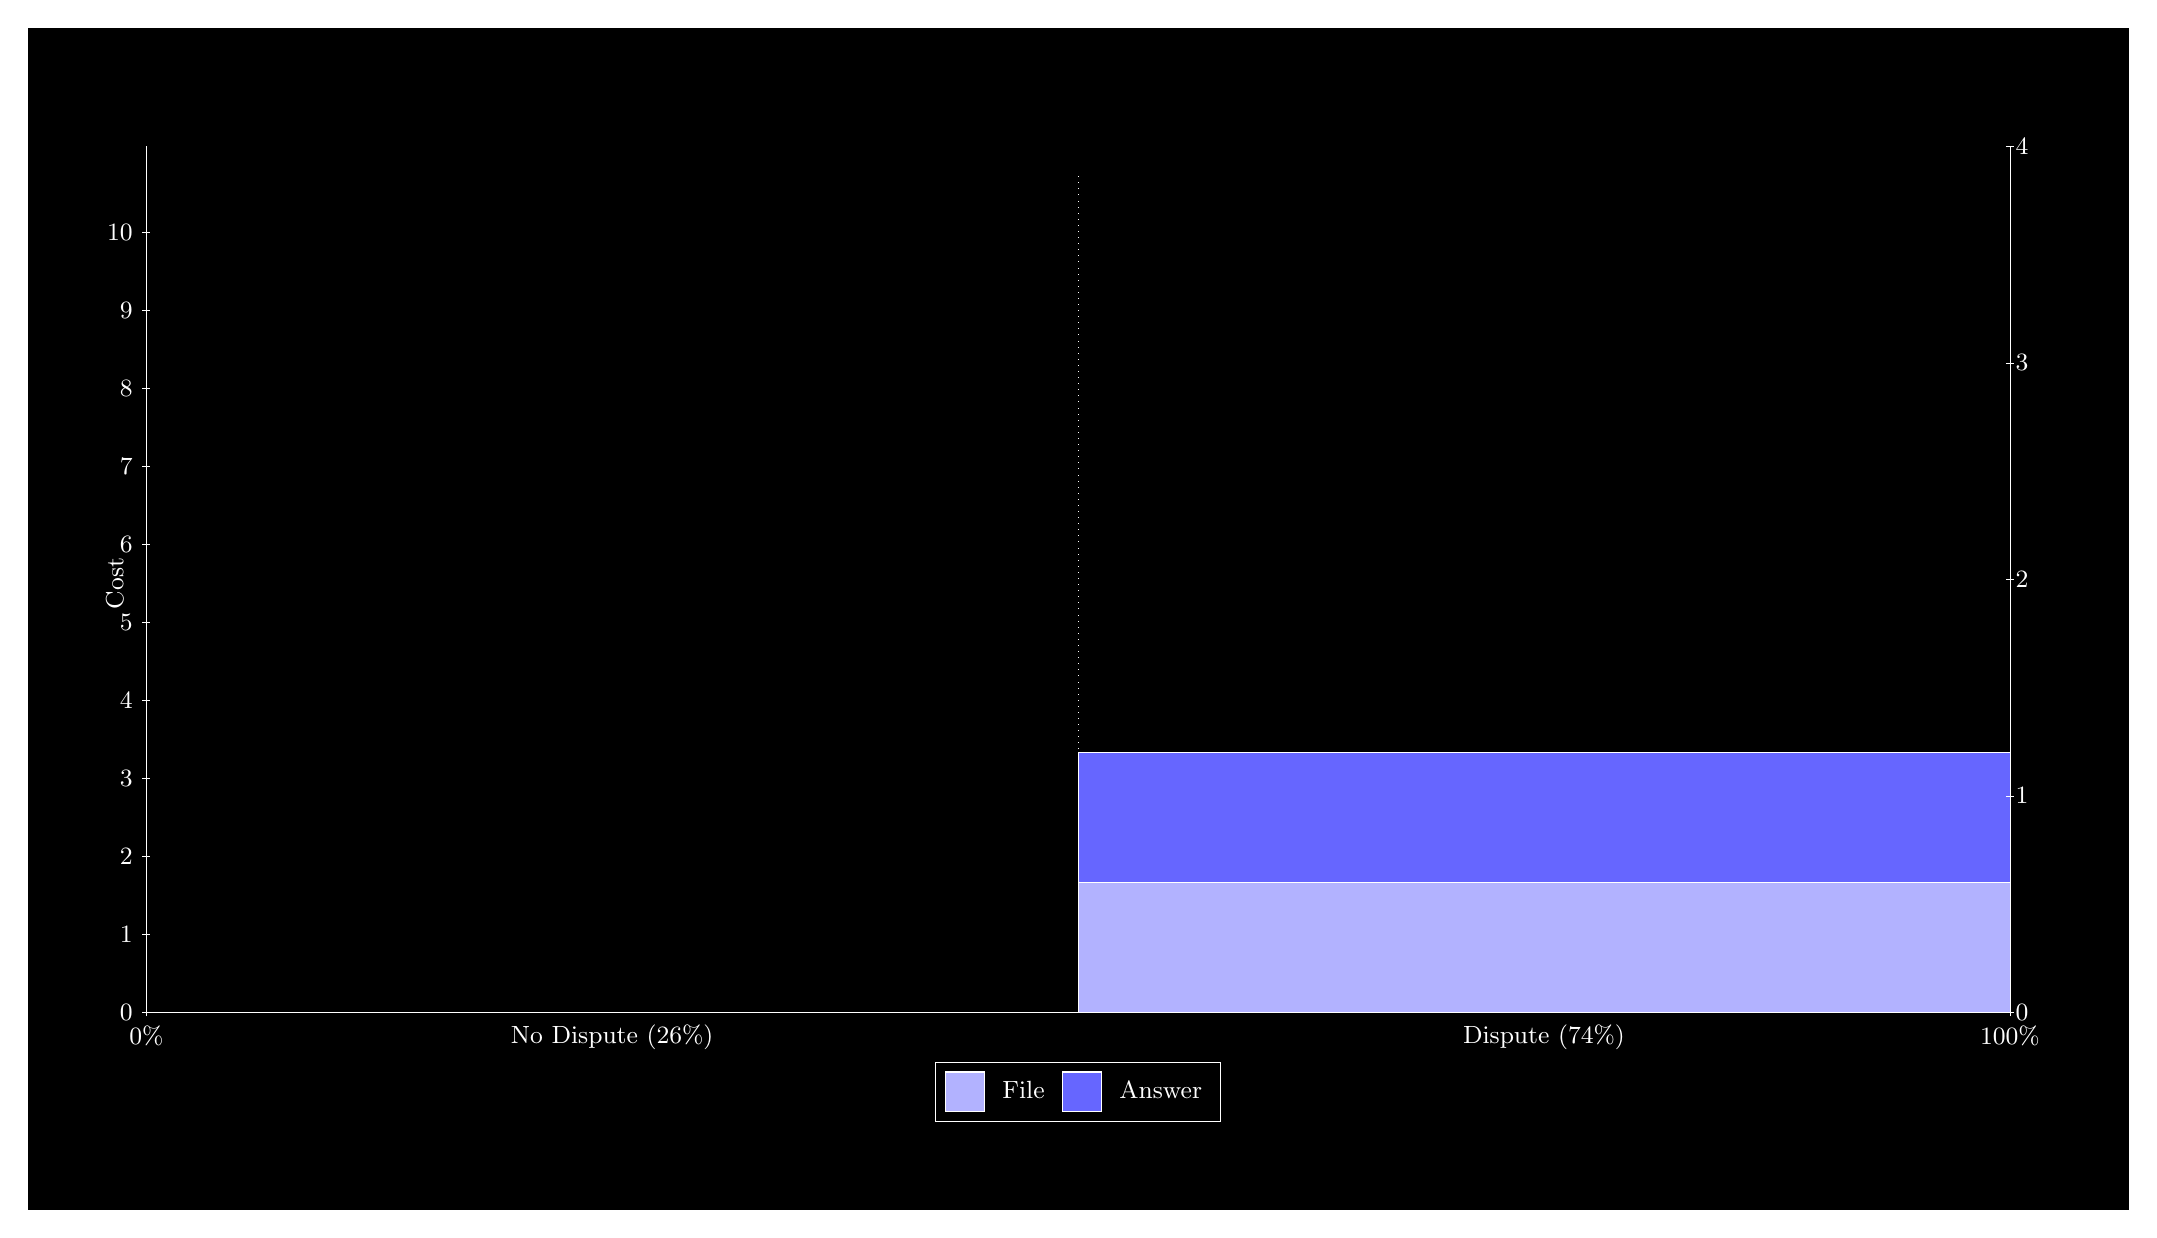
\begin{tikzpicture}
\draw[fill=black] (0,0) rectangle (26.667,15);
\draw[fill=blue!30,draw=white,very thin] (13.333,2.5) rectangle (25.167,4.15);
\draw[fill=blue!60,draw=white,very thin] (13.333,4.15) rectangle (25.167,5.8);
\draw[white,very thin] (1.5,2.5) -- (1.5,13.5);
\node[font=\small,rotate=90,text=white, anchor=center] at (1.1, 7.9497) {Cost};
\draw[white,very thin] (1.45,2.5) -- (1.55,2.5);
\node[font=\small,text=white, anchor=east] at (1.45, 2.5) {0};
\draw[white,very thin] (1.45,3.4908) -- (1.55,3.4908);
\node[font=\small,text=white, anchor=east] at (1.45, 3.4908) {1};
\draw[white,very thin] (1.45,4.4817) -- (1.55,4.4817);
\node[font=\small,text=white, anchor=east] at (1.45, 4.4817) {2};
\draw[white,very thin] (1.45,5.4725) -- (1.55,5.4725);
\node[font=\small,text=white, anchor=east] at (1.45, 5.4725) {3};
\draw[white,very thin] (1.45,6.4634) -- (1.55,6.4634);
\node[font=\small,text=white, anchor=east] at (1.45, 6.4634) {4};
\draw[white,very thin] (1.45,7.4542) -- (1.55,7.4542);
\node[font=\small,text=white, anchor=east] at (1.45, 7.4542) {5};
\draw[white,very thin] (1.45,8.4451) -- (1.55,8.4451);
\node[font=\small,text=white, anchor=east] at (1.45, 8.4451) {6};
\draw[white,very thin] (1.45,9.4359) -- (1.55,9.4359);
\node[font=\small,text=white, anchor=east] at (1.45, 9.4359) {7};
\draw[white,very thin] (1.45,10.427) -- (1.55,10.427);
\node[font=\small,text=white, anchor=east] at (1.45, 10.427) {8};
\draw[white,very thin] (1.45,11.418) -- (1.55,11.418);
\node[font=\small,text=white, anchor=east] at (1.45, 11.418) {9};
\draw[white,very thin] (1.45,12.408) -- (1.55,12.408);
\node[font=\small,text=white, anchor=east] at (1.45, 12.408) {10};

\draw[white,dotted,very thin] (13.333,2.83) -- (13.333,13.17);
\draw[white,very thin] (25.167,2.5) -- (25.167,13.5);
\draw[white,very thin] (25.117,2.5) -- (25.217,2.5);
\node[font=\small,text=white, anchor=west] at (25.117, 2.5) {0};
\draw[white,very thin] (25.117,5.25) -- (25.217,5.25);
\node[font=\small,text=white, anchor=west] at (25.117, 5.25) {1};
\draw[white,very thin] (25.117,8) -- (25.217,8);
\node[font=\small,text=white, anchor=west] at (25.117, 8) {2};
\draw[white,very thin] (25.117,10.75) -- (25.217,10.75);
\node[font=\small,text=white, anchor=west] at (25.117, 10.75) {3};
\draw[white,very thin] (25.117,13.5) -- (25.217,13.5);
\node[font=\small,text=white, anchor=west] at (25.117, 13.5) {4};

\draw[white,very thin] (1.5,2.5) -- (25.167,2.5);
\draw[white,very thin] (1.5,2.45) -- (1.5,2.55);
\node[font=\small,text=white, anchor=north] at (1.5, 2.45) {0\%};
\draw[white,very thin] (25.167,2.45) -- (25.167,2.55);
\node[font=\small,text=white, anchor=north] at (25.167, 2.45) {100\%};

\node[font=\small,text=white,anchor=south] at (7.4167, 1.9) {No\ Dispute\ (26\%)};
\node[font=\small,text=white,anchor=south] at (19.25, 1.9) {Dispute\ (74\%)};
\draw (13.3333,2.5) node (B) {};
\begin{scope}[align=center]
\matrix[scale=0.5,draw=white,below=0.5cm of B,nodes={draw},column sep=0.1cm]{
\node[rectangle,draw,minimum width=0.5cm,minimum height=0.5cm,fill=blue!30]{}; & \node[draw=none,font=\small,text=white]{File}; &
\node[rectangle,draw,minimum width=0.5cm,minimum height=0.5cm,fill=blue!60]{}; & \node[draw=none,font=\small,text=white]{Answer}; \\\\
};\end{scope}

\end{tikzpicture}
\end{document}